% symmetry in dynamical systems

We consider a system of \ode s of the form
\beq
	\dot{\ssp} = \vf(\ssp)
	\label{eq:difeq}
\eeq
where $\vf: \Rls{n} \rightarrow \Rls{n}$ a $C^\infty$ mapping.

We call a group element $\gamma\in\On{n}$ a symmetry of
\refeq{eq:difeq} if for every solution $x(t)$, $\gamma x(t)$
is also a solution. Equivalently $\gamma$ is a symmetry of \refeq{eq:difeq}:
\beq
	\vf(\gamma x) =\gamma \vf(x)
	\label{eq:equiv}
\eeq
for all $x\in\Rls{n}$. We say that $\vf$ \emph{commutes} with
$\gamma$ or that $\vf$ is $\gamma$-\emph{equivariant}. When
$\vf$ commutes with all $\gamma\in\Group$ we say that $\vf$
is $\Group$-equivariant. The finite time flow
$\flow{t}{\gamma x_o}$ through $\gamma x_o$ satisfies the
equivariance condition $\flow{t}{\gamma x_o}=\gamma
\flow{t}{x_o}$ from definition of symmetry and uniqueness of
solutions. In physics literature the term $invariant$ is most
commonly used, mostly because in Hamiltonian systems symmetry
is manifested as invariance of the Hamiltonian under the
symmetry operation.

\CLe\ are equivariant under the one parameter rotation
group $\Un{1}\cong\SOn{2}$ acting by
\beq
	(x,\,y,\,z)\mapsto (e^{i\theta}x,\,e^{i\theta}y,\,z)\,,\ \theta\in[0,2\pi]\,.
\eeq 
\ES{In this representation equivariance is easy to check but here we should
also discuss infinitesimal generator.}

The systems that we study here are not associated with a variational principle. Therefore
Noether's theorem does not apply and we  cannot conclude the existence of a conserved quantity associated
with a continuous symmetry of the system. Such a conserved quantity would restrict dynamical
trajectories to an invariant manifold locally transverse to the direction of group action.
In the contrary here the system also evolves along the direction of group action. In the example of {\CLe}
this is demonstrated in \reffig{fig:CLE}, where we project trajectories in $(x_1,x_2,z)$ axes, 
where $x=x_1+ i\, x_2\,,\ y=y_1+i\, x_2$ with $x_i,\,y_i\in\Rls{}$. In this projection a generic 
trajectory can be seen as one that traces a Lorenz-butterfly like attractor while at the same time slowly
``drifting'' along the direction of rotations. \refFig{fig:CLE} also illustrates the need for continuous symmetry 
reduction as a prerequisite for an understanding of state space geometry of such systems. 
The lowest level of organization of the familiar (real) Lorenz system that does not posses a continuous symmetry
can be understood\rf{DasBuch,SiminosThesis} in terms of the unstable manifolds of the equilibrium at the origin and the two (discrete-symmetry-related) equilibria $\EQB{1,2}$. In the case of {\CLE}  the origin \EQB{0} 
is an \eqv\ of \refeq{eq:CLe} for any
value of the parameters. As shown in \refref{FowlerCLE82} it
is stable for $0<\RerCLor<\rho_{1c}$ and unstable for
$\rho_{1c}<\RerCLor$, where
\beq
	\rho_{1c} = 1 + \frac{(e+\ImrCLor)(e-\sigma \ImrCLor)}{(\sigma+1)^2}\,.
\eeq
At bifurcation a pair of eigenvalues crosses the imaginary axis with imaginary part:
\beq
	\omega_c = \frac{\sigma (e + \ImrCLor)}{\sigma+1}\,.
	\label{eq:omegaCLE}
\eeq
and a \emph{relative equilibrium}, an equilibrium in a frame rotating with constant angular velocity
is born. Alternatively we might say that a relative equilibrium is a periodic orbit that is invariant (as a set)
under the action of \Gelement\ES{this implies constant angular velocity by equivariance.}.
\ES{Does not fit here, but keep: For $e+\ImrCLor=0$ the relative equilibrium degenerates to an \SOn{2}-orbit of \eqva\rf{FowlerCLE82}, since $\omega_c =0$.}  As we will see in \refsect{s:StabReq}, \REQB{1} of {\CLe} for 
the parameter set we study here is an unstable spiral, with one complex expanding eigenvalue. Yet, being a periodic
orbit, its unstable manifold is three-dimensional, with one eigendirection corresponding
to the direction of $\vf$ which also coinsides with the direction of rotations of the system. 
In \reffig{fig:CLE} we plot one trajectory on the unstable manifold of \REQB{1}. While it spirals away
from $\REQB{1}$ it also ``drifts'' along the direction of rotations of the system. This drifting motion obscures 
understanding of the stretching mechanism along the expanding eigendirection and subsequently the folding of the
unstable manifold back to itself.


The secondary bifurcation from the \reqv\ is expected according
to Krupa's theorem\rf{Krupa90} to result in
\emph{relative periodic orbits} that satisfy
\beq
	\LGelement{l}x(t+T_p)=x(t)\,,
\eeq
{\ie} they ``return'' after a time period $T_p$ to a point related to  . In the non-generic case of an
\SOn{2}-orbit of \eqva, again according to
Krupa\rf{Krupa90} theorem, one gets bifurcation
to periodic orbits. A secondary bifurcation has been
studied in \refref{NingHakenCLE90}.
    \ES{
The results are messy and hard to comment on. They show
existence of supercritical and subcritical bifurcations. Will
continue this discussion later}
Since we are interested in \CLe\
precisely for its symmetry properties we will concentrate on the
case that results to generic bifurcations. Before we proceed
with this, we briefly examine the special case $e=\ImrCLor=0$.

%
%%%%%%%%%%%%%%%%%%%%%%%%%%%%%%%%%%%%%%%%%%%%%%%%%%%%%%%%%%%%
\begin{figure}[ht]
\begin{center}
  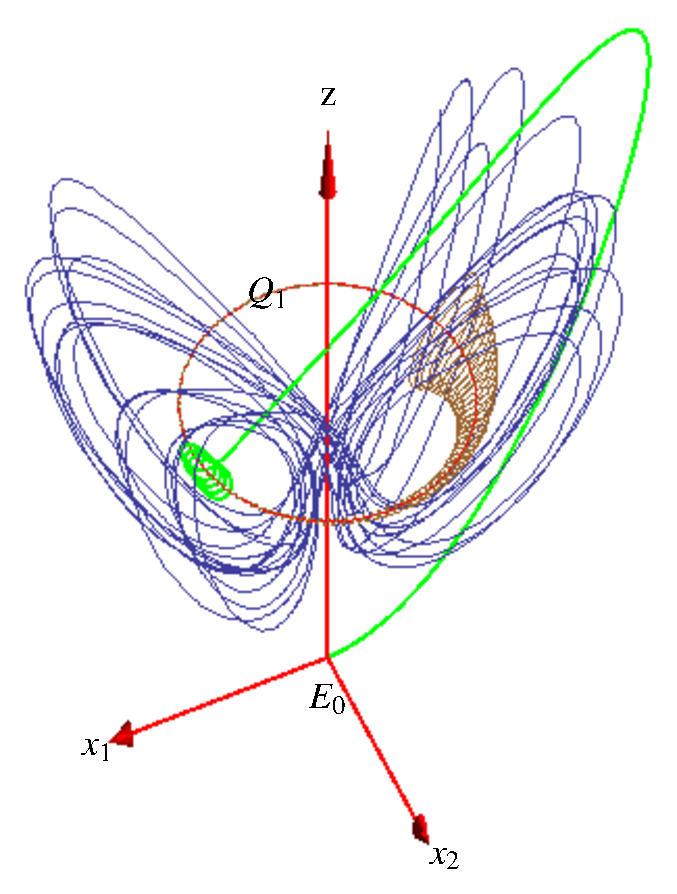
\includegraphics[height=0.25\textheight]{../figs/CLE}
\end{center}
\caption[Complex Lorenz flow phase space]
{ \Statesp\ portrait of \CLe\ dynamics for $e=1/10,\,
\ImrCLor=0$. Plotted are \reqv\ \REQB{1} (red), its unstable
manifold (brown), \eqv\ \EQB{0}, a representative of its
unstable manifold (green), 3 repetitions of \rpo\
``01''(magenta) and a generic orbit (blue).}
\label{fig:CLE}
\end{figure}
%%%%%%%%%%%%%%%%%%%%%%%%%%%%%%%%%%%%%%%%%%%%%%%%%%%%%%%%%%%%
%


